% =============================================================================
% Thoraxis - Informe del Proyecto Integrador
% Programa en Deep Learning - UTEC Posgrado
% =============================================================================
% Único punto de entrada. El orden de las partes es el de la sección 3
% ("Estructura del Trabajo Final") de la guía del proyecto integrador:
%
%   3.1  Portada                      sections/00-cover.tex
%   3.2  Resumen ejecutivo (1 pág.)   sections/01-executive-summary.tex
%   3.3  Introducción                 sections/02-introduction.tex
%   3.4  Datos y preparación          sections/03-data.tex
%   3.5  Desarrollo de la solución    sections/04-development.tex
%   3.6  Evaluación de la solución    sections/05-evaluation.tex
%   3.7  Resultados y discusión       sections/06-results-discussion.tex
%   3.8  Conclusiones                 sections/07-conclusions.tex
%   3.9  Referencias                  bibliography/references.bib (IEEE)
%
% Para compilar con el nombre final (thoraxis-article.pdf) usar
% scripts/build.ps1 o scripts/build.sh, que también ejecutan biber.
% =============================================================================

% !TEX root = ../article.tex
% =============================================================================
% Preamble - Clase, paquetes y formato del informe
% Thoraxis - Proyecto Integrador del Programa en Deep Learning (UTEC Posgrado)
% =============================================================================
% Artículo a una sola columna, sin límite de páginas. La guía del proyecto
% integrador (Documentos/Proyecto-Integrador-Grupal-Deep-Learning.pdf) fija
% las secciones y que solo el resumen ejecutivo no exceda una página, pero no
% el formato visual.
% El aspecto (Century Schoolbook) se toma de la tesis del
% autor (github.com/ahincho/thesis) para mantener un estilo propio y
% coherente.
%
% Todo lo que define el aspecto vive en este archivo; el texto vive en
% sections/.
% =============================================================================

\documentclass[11pt, a4paper, oneside, onecolumn]{article}

% --- Codificación ---
% Los .tex se escriben en UTF-8 con acentos directos, sin \'a.
\usepackage[utf8]{inputenc}
\usepackage[T1]{fontenc}

% --- Idioma ---
%   es-noquoting     desactiva el " activo de babel-spanish (choca con tablas)
%   es-tabla         "Tabla" en lugar de "Cuadro"
%   es-nodecimaldot  no cambia el punto decimal en modo matemático
\usepackage[english, spanish, es-noquoting, es-tabla, es-nodecimaldot]{babel}

% --- Geometría de página ---
% headheight da espacio al logo del encabezado (\articleHeaderLogoHeight).
\usepackage[top=2.5cm, bottom=2.5cm, left=2.5cm, right=2.5cm, headheight=22pt]{geometry}

% --- Tipografía ---
% TeX Gyre Schola (Century Schoolbook) con matemáticas a juego.
\usepackage{tgschola}
\usepackage[nc]{newtxmath}
\usepackage{microtype}

% --- Interlineado y párrafos ---
\usepackage{setspace}
\setstretch{1.15}
\setlength{\parindent}{1.25em}
\setlength{\parskip}{0.3em}

% Válvula de escape contra Overfull \hbox en términos técnicos largos.
\setlength{\emergencystretch}{1.5em}
\hyphenation{PyTorch MONAI FastAPI NiiVue Cornerstone Evidently GitHub
    ReproPath Thoraxis}

% --- Colores ---
\usepackage{xcolor}
\definecolor{articlegray}{gray}{0.35}   % Títulos de sección
\definecolor{articlelink}{HTML}{0B5394} % Enlaces

% --- Gráficos ---
\usepackage{graphicx}
\graphicspath{{figures/}}
% Los diagramas se hacen con Excalidraw y se insertan como PDF (ver diagrams/).

% --- Títulos de secciones ---
\usepackage{titlesec}
\titleformat{\section}{\normalfont\Large\bfseries\color{articlegray}}{\thesection.}{0.6em}{}
\titleformat{\subsection}{\normalfont\large\bfseries}{\thesubsection.}{0.6em}{}
\titleformat{\subsubsection}{\normalfont\normalsize\bfseries}{\thesubsubsection.}{0.6em}{}
\titlespacing*{\section}{0pt}{1.4em}{0.8em}
\titlespacing*{\subsection}{0pt}{1.1em}{0.5em}
\setcounter{secnumdepth}{3}
\setcounter{tocdepth}{2}

% --- Encabezados y pies ---
% A la izquierda, "Proyecto Integrador -- Thoraxis"; a la derecha, el programa
% y el logo de UTEC Posgrado; al pie, el número de página. La portada no lleva
% encabezado (titlepage).
%
% El logo se apoya en la línea base, para no tocar la línea del encabezado, y
% \articleHeaderText sube los dos textos hasta el centro del logo: la mitad
% de la altura del logo menos la mitad de la altura de la "P". Así el texto y
% el logo quedan a la misma altura, los textos de ambos lados siguen
% alineados entre sí y el centrado se mantiene aunque cambie el tamaño del
% logo o de la letra.
\newcommand{\articleHeaderText}[1]{%
    \raisebox{\dimexpr 0.5\articleHeaderLogoHeight - 0.5\fontcharht\font`P\relax}{#1}}
\usepackage{fancyhdr}
\fancypagestyle{article}{%
    \fancyhf{}%
    \fancyhead[L]{\footnotesize\articleHeaderText{\articleDocument{} -- \articleShortTitle}}%
    \fancyhead[R]{\footnotesize\articleHeaderText{\articleProgram}\hspace{0.8em}%
        
\includegraphics[height=\articleHeaderLogoHeight]{utec-posgrado}}%
    \fancyfoot[C]{\thepage}%
    \renewcommand{\headrulewidth}{0.4pt}%
}

% --- Figuras y tablas ---
\usepackage{float}          % [H] para fijar una figura en su lugar
\usepackage{array}
\usepackage{tabularx}
\usepackage{booktabs}
\usepackage{multirow}
% Más aire entre filas de las tablas, para que las de varias líneas no se
% junten.
\renewcommand{\arraystretch}{1.25}
\usepackage[
    labelfont=bf,
    labelsep=period,
    font=small,
    justification=centering,
    singlelinecheck=false,
    skip=6pt
]{caption}

% --- Listas ---
\usepackage{enumitem}
\setlist{itemsep=0.2em, topsep=0.4em}

% --- Matemáticas y unidades ---
\usepackage{amsmath}
\usepackage{siunitx}
\sisetup{output-decimal-marker={,}, group-separator={\,}}

% --- Páginas horizontales para figuras anchas ---
% pdflscape gira la página en el visor de PDF, además de en la impresión.
\usepackage{pdflscape}
\usepackage{afterpage}

% --- Control de extensión del resumen ejecutivo ---
% refcount lee los números de página de las etiquetas (ver commands.tex).
\usepackage{refcount}

% --- Bibliografía (IEEE) ---
% Estilo numérico IEEE (biblatex-ieee): las referencias se numeran en el orden
% en que se citan. \parencite{clave} da [n] y \textcite{clave}, «Autor et al. [n]».
\usepackage{csquotes}
\usepackage[style=ieee, backend=biber]{biblatex}
\addbibresource{bibliography/references.bib}
% IEEE usa raya corta (en dash) en los rangos de páginas; el estilo en español
% pone un guion.
\DefineBibliographyExtras{spanish}{\renewcommand*{\bibrangedash}{\textendash}}
% biblatex-ieee solo trae sus textos en inglés: estos son sus equivalentes en
% español (número de artículo, fecha de consulta y dirección web).
\DefineBibliographyStrings{spanish}{%
    artno   = {art\adddot\addnbspace n\adddot\textsuperscript{o}},
    urlseen = {Consultado\addcolon},
    url     = {Disponible en},
}

% --- Enlaces ---
% hyperref va casi al final: redefine comandos de los paquetes anteriores.
\PassOptionsToPackage{hyphens}{url}
\usepackage[
    colorlinks=true,
    linkcolor=black,
    citecolor=black,
    urlcolor=articlelink,
    bookmarksnumbered=true,
    pdfborder={0 0 0}
]{hyperref}
\urlstyle{same}
     % Clase, paquetes y formato
% !TEX root = ../article.tex
% =============================================================================
% Metadatos del informe
% =============================================================================
% Todo lo que aparece en la portada (sección 3.1 de la guía), en el
% encabezado y en las propiedades del PDF. Cambiar un dato aquí lo actualiza
% en todos los lugares donde se usa.
% =============================================================================

% --- Programa ---
\newcommand{\articleInstitution}{Universidad de Ingeniería y Tecnología (UTEC) -- Posgrado}
\newcommand{\articleProgram}{Programa en Deep Learning}
\newcommand{\articleDocument}{Proyecto Integrador}
\newcommand{\articleLeaderLabel}{Líder Académico}
\newcommand{\articleLeader}{Victor Flores Benites}
% Ancho del logo de UTEC Posgrado en la portada y alto en el encabezado. Si
% el del encabezado crece, subir también headheight en config/preamble.tex.
% El alto del encabezado es una longitud (\setlength) y no una macro, porque
% se usa en cálculos: "0.5\articleHeaderLogoHeight" con una macro "16pt" se
% leería como 0.516pt.
\newcommand{\articleLogoWidth}{9cm}
\newcommand{\articleLogoTopSpace}{2.5cm}
\newlength{\articleHeaderLogoHeight}
\setlength{\articleHeaderLogoHeight}{16pt}

% Fecha de entrega. La final es el sábado 20 de marzo de 2027; para cada
% avance, cambiarla por la fecha de la asesoría correspondiente.
\newcommand{\articleDate}{20 de marzo de 2027}

% --- Trabajo ---
\newcommand{\articleTitle}{Thoraxis: Segmentación de Estructuras del Tórax
    en Tomografía Computarizada con Deep Learning}
\newcommand{\articleShortTitle}{Thoraxis}
\newcommand{\articleDisclaimer}{Herramienta de investigación. No está
    destinada al diagnóstico clínico.}

% --- Integrantes ---
% La guía pide equipos de tres integrantes con nombres completos.
\newcommand{\articleAuthors}{%
    Angel Eduardo Hincho Jove\\
    \pendiente{integrante 2}\\
    \pendiente{integrante 3}%
}
% Versión sin marcas para las propiedades del PDF.
\newcommand{\articleAuthorsPDF}{Angel Eduardo Hincho Jove}

% --- Palabras clave (resumen ejecutivo y metadatos del PDF) ---
\newcommand{\articleKeywords}{Deep Learning, Integración Continua, Entrega Continua,
    Despliegue Continuo, MLOps, Segmentación de Imágenes Médicas, Tomografía Computarizada,
    Tórax, Pulmón, Reproducibilidad, Explicabilidad}
     % Título, integrantes, programa, fecha
% !TEX root = ../article.tex
% =============================================================================
% Macros propias y metadatos del PDF
% =============================================================================

% --- Metadatos del PDF ---
\hypersetup{
    pdftitle={\articleTitle},
    pdfauthor={\articleAuthorsPDF},
    pdfsubject={\articleDocument{} - \articleProgram, \articleInstitution},
    pdfkeywords={\articleKeywords},
    pdflang={es-PE}
}

% --- Fuente de figuras y tablas ---
% Debajo de cada figura o tabla:
%   \articleSource{Elaboración propia.}
%   \articleSource{Adaptado de \textcite{clave}.}
\newcommand{\articleSource}[1]{%
    \par\vspace{0.3em}%
    {\footnotesize\centering\textit{Fuente:} #1\par}%
}

% --- Notas mientras se escribe ---
% \pendiente{...} marca en rojo lo que falta. Antes de entregar no debe
% quedar ninguno: los scripts de compilación avisan cuántos hay.
\newcommand{\pendiente}[1]{\textcolor{red}{[PENDIENTE: #1]}}

% --- Resumen ejecutivo de una página ---
% La guía pide que no exceda una página. sections/01-executive-summary.tex
% pone \label{summary:start} y \label{summary:end}; si caen en páginas
% distintas, LaTeX emite un aviso que los scripts de compilación muestran.
% El aviso dice "hoja" y no "página" a propósito: pdflatex no escribe bien
% las tildes en el .log, y los scripts buscan este texto exacto.
\newcommand{\articleCheckOnePage}{%
    \ifnum\getpagerefnumber{summary:end}>\getpagerefnumber{summary:start}\relax
        \PackageWarningNoLine{thoraxis}{El resumen ejecutivo excede una hoja}%
    \fi
}
     % Macros propias y metadatos del PDF

\begin{document}

% !TEX root = ../article.tex
% =============================================================================
% 3.1 Portada
% =============================================================================
% La guía pide: título del proyecto, nombres completos de los integrantes,
% nombre del programa y del líder académico, y fecha de entrega. Los datos
% salen de config/metadata.tex.
%
% El logo (figures/utec-posgrado.png) se extrajo de la guía oficial del
% proyecto integrador, que es la versión que UTEC usa en sus documentos del
% programa. Su tamaño se cambia en \articleLogoWidth (config/metadata.tex).
% =============================================================================

\begin{titlepage}
    \centering
    % Espacio sobre el logo; los \vfill de abajo reparten el resto de la hoja.
    \vspace*{\articleLogoTopSpace}
    
\includegraphics[width=\articleLogoWidth]{utec-posgrado}\par
    \vspace{1.5em}
    {\large\articleInstitution\par}
    \vspace{0.4em}
    {\large\articleProgram\par}
    \vspace{0.4em}
    {\normalsize\scshape\articleDocument\par}

    \vfill

    {\LARGE\bfseries\articleTitle\par}
    \vspace{1em}
    {\small\textit{\articleDisclaimer}\par}

    \vfill

    {\large\bfseries Integrantes\par}
    \vspace{0.5em}
    {\large\articleAuthors\par}

    \vspace{2.5em}

    {\large\bfseries\articleLeaderLabel\par}
    \vspace{0.5em}
    {\large\articleLeader\par}

    \vfill

    {\large\articleDate\par}
\end{titlepage}


\pagestyle{article}
% !TEX root = ../article.tex
% =============================================================================
% 3.2 Resumen ejecutivo
% =============================================================================
% La guía pide: descripción del problema, la solución desarrollada, los datos
% utilizados y los principales resultados. Debe permitir comprender el aporte
% del proyecto y NO EXCEDER UNA PÁGINA. Si se pasa, los scripts de
% compilación lo avisan (ver \articleCheckOnePage en config/commands.tex).
%
% Versión del primer avance: resume lo redactado en las secciones 1 a 3. Los
% resultados se completan cuando existan y el resto se ajusta tras cada
% asesoría.
% =============================================================================

\section*{Resumen ejecutivo}
\addcontentsline{toc}{section}{Resumen ejecutivo}
\label{summary:start}

\paragraph{Problema.}
Las enfermedades pulmonares están entre las principales causas de muerte en el
mundo: en 2023, la EPOC fue la tercera, y en 2024 el cáncer de pulmón fue el
más diagnosticado, con casi 2,6 millones de casos nuevos
\parencite{oms2026, sung2026}. La tomografía computarizada permite medirlas,
pero para cuantificar el volumen pulmonar o la extensión de una lesión primero
hay que delimitar el pulmón. Hacerlo a mano toma horas por estudio, los métodos
clásicos fallan cuando el pulmón tiene patología, y los modelos publicados son
difíciles de comparar y de reproducir.

\paragraph{Solución.}
Thoraxis segmenta automáticamente el pulmón izquierdo y el derecho en
tomografías de tórax con Deep Learning y calcula el volumen de cada uno. La
solución base es una U-Net 2D que procesa cada corte por separado; la propuesta
agrega contexto entre cortes contiguos (2.5D), aumentos de datos y datos de
entrenamiento más diversos. El modelo elegido se exporta a ONNX y se sirve con
una API en FastAPI, que alimenta un visor web con la máscara superpuesta y un
mapa de incertidumbre que muestra dónde el modelo es menos confiable. El
ciclo de vida sigue prácticas de MLOps: experimentos en MLflow sobre
Databricks, datos versionados con DVC, integración continua con GitHub Actions,
reentrenamiento en Kaggle, monitoreo de la deriva con Evidently y del
rendimiento de la API con OpenTelemetry y Grafana.

\paragraph{Datos.}
Se usan tres conjuntos públicos y anonimizados con máscaras de ambos pulmones.
Para entrenar, validar y probar se combinan TotalSegmentator, con 1939
tomografías de rutina clínica, y 20 tomografías de pacientes con COVID-19. La
validación externa se hace con LCTSC: 60 pacientes con cáncer de pulmón de tres
instituciones, que no se usan para entrenar. Toda partición se hace
por paciente, y ningún dato médico se guarda en los repositorios.

\paragraph{Resultados esperados.}
El proyecto se considerará exitoso si la propuesta alcanza un coeficiente de
Dice medio de al menos 0,95 por pulmón en la validación externa, supera a la
solución base con un intervalo de confianza que excluya el cero, funciona de
extremo a extremo en el prototipo y su evaluación puede reproducirse desde los
repositorios.
\pendiente{métricas obtenidas por la propuesta y la solución base}

\paragraph{Aporte y limitaciones.}
Thoraxis aporta un modelo de segmentación pulmonar portable, explicado con
mapas de incertidumbre en lugar de mapas de calor poco confiables, y una
evaluación reproducible, con validación externa e intervalos de confianza. Es
una
herramienta de investigación y no un sistema de diagnóstico: se evalúa solo con
datos públicos, sin validación clínica, y las diferencias en cómo cada conjunto
delimita el pulmón pueden afectar sus métricas.

\medskip
\noindent\textbf{Palabras clave:} \articleKeywords.

\label{summary:end}
\articleCheckOnePage


\clearpage
% !TEX root = ../article.tex
% =============================================================================
% 3.3 Introducción
% =============================================================================
% Guía: contexto del problema y razones para abordarlo; usuarios o procesos
% que se beneficiarían; objetivo general, objetivos específicos y alcance;
% resultado esperado y forma de comprobar si se ha alcanzado.
%
% Primer avance (asesoría 1, 6-13 nov 2026): problema seleccionado, contexto
% y evidencia inicial, objetivos y resultados esperados.
% =============================================================================

\section{Introducción}\label{sec:introduction}

% Cifras y afirmaciones verificadas en los resúmenes de cada fuente (Crossref
% y PubMed) el 8 de noviembre de 2026.
\subsection{Contexto y motivación}\label{sec:context}
Las enfermedades pulmonares están entre las principales causas de muerte en el
mundo. En 2023, tres de las diez primeras afectaron al pulmón: la enfermedad
pulmonar obstructiva crónica (EPOC), tercera con unos 3,6 millones de muertes;
las infecciones de las vías respiratorias inferiores, cuarta con 2,7 millones;
y el cáncer de tráquea, bronquios y pulmón, séptima con 1,8 millones
\parencite{oms2026}. El cáncer de pulmón fue además, en 2024, el cáncer
diagnosticado con más frecuencia, con casi 2,6 millones de casos nuevos, y la
primera causa de muerte por cáncer, con unos 1,9 millones de fallecimientos
\parencite{sung2026}.

La tomografía computarizada (TC) permite examinar el pulmón en tres
dimensiones y medirlo. La TC cuantitativa traduce la imagen en medidas
numéricas automáticas, y una revisión sistemática de 185 estudios encontró que
estas medidas aportan información pronóstica en las enfermedades pulmonares
intersticiales \parencite{dixon2025}. Para obtenerlas, primero hay que separar
el pulmón del resto del tórax; esa delimitación, llamada segmentación, es un
paso crucial del análisis de imagen \parencite{hofmanninger2020}. En la
fibrosis pulmonar idiopática, por ejemplo, un modelo de Deep Learning segmentó
con éxito el 97,8~\% de las TC, de distintos fabricantes y con espesores de
corte de 0,5 a 5~mm. En una cohorte de 446 pacientes, el volumen pulmonar
obtenido se correlacionó con la capacidad vital forzada ($r = 0{,}82$), y un
volumen menor se asoció con una menor supervivencia libre de progresión a dos
años \parencite{thillai2024}.

Estas medidas, sin embargo, todavía no se usan de forma rutinaria en la
práctica clínica ni en los ensayos \parencite{thillai2024}, y no están
estandarizadas: la heterogeneidad de los métodos impidió comparar entre sí los
estudios de la revisión o combinarlos en un metaanálisis \parencite{dixon2025}.
Los métodos automáticos clásicos, basados en umbrales, regiones o formas, no
resuelven el problema, porque casi todos funcionan bien solo cuando el pulmón
presenta poca o ninguna patología; derrames pleurales, consolidaciones y masas
provocan segmentaciones inexactas \parencite{mansoor2015}. Delimitar el pulmón
a mano tampoco es viable en la rutina: en el conjunto de \textcite{ma2021},
delimitar el pulmón y la infección en una TC de 250 cortes tomó en promedio
unos 400 minutos. Además, reunir grandes conjuntos de imágenes anotadas en una
sola institución es poco práctico, sobre todo cuando los radiólogos están
dedicados a la atención \parencite{ma2021}.

El aprendizaje profundo ha cambiado este panorama. Con 70 casos de COVID-19
anotados, \textcite{ma2021} obtienen un coeficiente de Dice promedio de 97,3~\%
y 97,7~\% para el pulmón izquierdo y el derecho, aunque solo de 67,3~\% para la
infección. \textcite{hofmanninger2020} muestran que, en casos difíciles, la
precisión depende más de la diversidad de los datos de entrenamiento que de la
arquitectura: una U-Net entrenada con datos clínicos de rutina de varias
enfermedades alcanza un Dice de 0,98, frente a 0,94 de los métodos de
referencia. TotalSegmentator, un modelo nnU-Net entrenado con 1204 estudios de
TC de rutina, segmenta 104 estructuras anatómicas, con usos como la volumetría de órganos y la planificación de
radioterapia \parencite{wasserthal2023}. Persisten, no obstante, dos
dificultades: los métodos son difíciles de comparar porque se desarrollan con
datos, configuraciones y métricas distintos \parencite{ma2021}, y la
variabilidad propia del entrenamiento pone en duda la reproducibilidad de sus
resultados \parencite{renard2020}.

Thoraxis aborda la segmentación pulmonar en TC por cuatro razones:

\begin{enumerate}
    \item \textbf{Relevancia:} la segmentación del pulmón es el paso previo
          para cuantificar enfermedades con una carga sanitaria alta.
    \item \textbf{Viabilidad:} existen conjuntos de datos públicos con máscaras
          de referencia y modelos publicados que sirven como referencia, lo
          que permite evaluar la propuesta en condiciones comparables.
    \item \textbf{Brecha:} la robustez ante pulmones con patología y una
          evaluación reproducible y verificable siguen siendo problemas
          abiertos.
    \item \textbf{Proyección:} el pulmón es el primer caso; la misma
          infraestructura de entrenamiento, evaluación y despliegue puede
          extenderse a otras estructuras del tórax.
\end{enumerate}

Thoraxis es una herramienta de investigación y no un sistema de diagnóstico:
sus resultados no reemplazan la evaluación de un especialista.
\pendiente{evidencia local, si el equipo la incorpora: acceso a TC o a
radiólogos en el Perú}

\subsection{Usuarios y procesos beneficiados}\label{sec:users}
Thoraxis está pensado para usuarios del ámbito de la investigación, en cuatro
procesos:

\begin{itemize}
    \item \textbf{Equipos de investigación en imagen médica} que analizan
          cohortes retrospectivas de TC y necesitan medir el volumen de cada
          pulmón en muchos estudios, sin delimitarlos uno por uno.
    \item \textbf{Radiólogos y anotadores} que preparan conjuntos de datos: en
          lugar de trazar el pulmón desde cero, una tarea que puede tomar horas
          por estudio \parencite{ma2021}, revisan y corrigen la máscara que
          propone el modelo.
    \item \textbf{Desarrolladores de otros modelos}, como detectores de nódulos
          o de lesiones, que necesitan el pulmón delimitado como paso previo
          de su análisis \parencite{hofmanninger2020}.
    \item \textbf{Desarrolladores de sistemas} que quieren integrar la
          segmentación en sus aplicaciones: el modelo se distribuye en ONNX y
          se expone mediante una API, de modo que puede ejecutarse desde otros
          lenguajes y marcos.
\end{itemize}

\noindent En todos los casos, el resultado lo revisa una persona. Thoraxis no
está dirigido a la atención de pacientes: usarlo en la práctica clínica
exigiría una validación clínica y las autorizaciones sanitarias
correspondientes, que quedan fuera del alcance del proyecto.

\subsection{Objetivos}\label{sec:objectives}

\paragraph{Objetivo general.}
Desarrollar y evaluar de forma reproducible un modelo de Deep Learning que
segmente automáticamente el pulmón izquierdo y el derecho en tomografías
computarizadas de tórax, incluidos pulmones con patología, e integrarlo en un
prototipo que muestre la segmentación y calcule el volumen de cada pulmón.

\paragraph{Objetivos específicos.}
\begin{enumerate}
    \item Preparar un conjunto de TC de tórax de fuentes públicas, con máscaras
          de referencia de ambos pulmones, un preprocesamiento homogéneo y una
          partición por paciente sin fugas entre entrenamiento, validación y
          prueba.
    \item Implementar una solución base, una U-Net 2D entrenada corte por
          corte, y una propuesta que la mejore con contexto entre cortes
          contiguos, aumentos de datos y datos de entrenamiento más diversos.
    \item Evaluar ambas soluciones en las mismas condiciones, con el
          coeficiente de Dice y la distancia de Hausdorff al percentil 95
          (HD95) e intervalos de confianza por \textit{bootstrap}, en una
          prueba interna y en una validación externa con datos de otras
          instituciones, usando TotalSegmentator como referencia publicada.
    \item Analizar los errores de la propuesta, en especial en pulmones con
          patología, identificar sus limitaciones y estimar la incertidumbre de
          cada segmentación para explicar dónde y cuándo el modelo es menos
          confiable.
    \item Exportar el modelo a ONNX y desplegarlo en un servicio de inferencia
          y un visor web que muestren la máscara sobre los cortes y el volumen
          de cada pulmón.
    \item Registrar los experimentos, configuraciones y versiones con MLflow,
          de modo que la evaluación pueda reproducirse desde los
          repositorios.
\end{enumerate}

\subsection{Alcance}\label{sec:scope}
El proyecto incluye:

\begin{itemize}
    \item Tomografías computarizadas de tórax de conjuntos de datos públicos y
          anonimizados, descritos en la Sección~\ref{sec:data}.
    \item La segmentación del pulmón izquierdo y del derecho, con modelos que
          procesan cortes individuales (2D) o pilas de cortes contiguos
          (2.5D).
    \item El cálculo del volumen de cada pulmón a partir de la máscara y del
          tamaño del vóxel.
    \item Un mapa de incertidumbre por vóxel y una puntuación de confianza por
          estudio, como forma de explicabilidad.
    \item Un prototipo con un servicio de inferencia y un visor web para
          cargar un estudio de prueba y revisar el resultado.
\end{itemize}

\noindent El proyecto no incluye:

\begin{itemize}
    \item La segmentación de lesiones, como la infección por COVID-19 o los
          nódulos, ni de los lóbulos u otras estructuras del tórax, que quedan
          como extensiones futuras.
    \item El diagnóstico, la clasificación de enfermedades o cualquier
          recomendación clínica.
    \item El uso con datos de pacientes fuera de los conjuntos públicos, la
          validación clínica prospectiva y la certificación como dispositivo
          médico.
    \item Otras modalidades de imagen, como la radiografía de tórax o la
          resonancia magnética.
\end{itemize}

\subsection{Resultado esperado y criterio de éxito}\label{sec:expected-outcome}
El resultado esperado es un modelo de segmentación de ambos pulmones,
exportado a ONNX y versionado, un prototipo que lo usa, y el código, las
configuraciones y los registros necesarios para reproducir su evaluación. Se
considerará alcanzado si se cumplen los siguientes criterios:

\begin{enumerate}
    \item \textbf{Exactitud externa:} el Dice medio por paciente es de al
          menos 0,95 para cada pulmón en la validación externa, reportado con
          su intervalo de confianza del 95~\%.
    \item \textbf{Mejora frente a la base:} la propuesta supera a la solución
          base en Dice en la prueba interna y en la externa, y el intervalo de
          confianza de la diferencia por pares no incluye el cero. La HD95 se
          reporta y se compara de la misma forma.
    \item \textbf{Prototipo funcional:} el prototipo procesa un estudio de
          prueba de extremo a extremo y muestra la máscara y el volumen de cada
          pulmón.
    \item \textbf{Reproducibilidad:} otro integrante del equipo reproduce la
          evaluación desde los repositorios y obtiene las mismas métricas.
\end{enumerate}

% !TEX root = ../article.tex
% =============================================================================
% 3.4 Datos y preparación
% =============================================================================
% Guía: origen, tamaño y características de los datos; criterios de
% selección, limpieza, etiquetado y preprocesamiento; separación de
% entrenamiento, validación y prueba (con modelos preentrenados, un conjunto
% de evaluación separado de los ejemplos usados para ajustar la solución);
% limitaciones de calidad o cobertura y tratamiento de información sensible.
%
% Primer avance: datos disponibles o fuente prevista y cómo se accederá a
% ellos.
%
% Datos de cada conjunto verificados el 8 de noviembre de 2026 en Zenodo
% (API de registros), en la página de la colección en TCIA, en el artículo de
% cada conjunto y en el repositorio del benchmark de COVID-19.
% =============================================================================

\section{Datos y preparación}\label{sec:data}

\subsection{Origen y características}\label{sec:data-source}
Thoraxis usa tres conjuntos públicos de TC de tórax con máscaras de referencia
de ambos pulmones, todos anonimizados por sus autores
(Tabla~\ref{tab:datasets}).

\begin{itemize}
    \item \textbf{TotalSegmentator}, versión~3: 1939 TC tomadas al azar de la
          rutina clínica y reunidas por el Hospital Universitario de Basilea,
          con una amplia variedad de
          patologías, equipos, secuencias e instituciones, y 117 estructuras
          segmentadas \parencite{wasserthal2023dataset}. La versión~3 agregó
          291 estudios pediátricos. Los pulmones están segmentados por
          lóbulos, con la tráquea como clase aparte \parencite{wasserthal2023}.
    \item \textbf{COVID-19 CT Lung and Infection Segmentation}: 20 TC de
          pacientes con COVID-19 de la Coronacases Initiative y de
          Radiopaedia, con el pulmón izquierdo, el derecho y la infección
          delimitados corte por corte \parencite{ma2020}. Anotadores con uno a
          cinco años de experiencia trazaron las máscaras, dos radiólogos las
          refinaron y un radiólogo con más de diez años de experiencia en
          tórax las verificó \parencite{ma2021}.
    \item \textbf{LCTSC} (\textit{Lung CT Segmentation Challenge} 2017): 60
          TC de planificación de radioterapia de pacientes con cáncer de
          pulmón, 20 de cada una de tres instituciones, con los contornos
          clínicos de pulmón izquierdo, pulmón derecho, corazón, esófago y
          médula espinal, revisados según la guía RTOG~1106
          \parencite{yang2017, yang2018}.
\end{itemize}

\begin{table}[htbp]
    \centering
    \caption{Conjuntos de datos de Thoraxis.}\label{tab:datasets}
    \small
    \begin{tabularx}{\textwidth}{>{\raggedright\arraybackslash}p{3cm}
                                 >{\raggedright\arraybackslash}p{1.4cm}
                                 >{\raggedright\arraybackslash}X
                                 >{\raggedright\arraybackslash}X
                                 >{\raggedright\arraybackslash}p{2.7cm}}
        \toprule
        Conjunto & Estudios & Formato, tamaño y acceso & Licencia & Uso en
            Thoraxis \\
        \midrule
        TotalSegmentator v3 & 1939 & 37,4~GB en Zenodo, descarga directa. &
            CC BY 4.0. & Entrenamiento, validación y prueba interna. \\
        COVID-19 CT Lung and Infection & 20 & NIfTI; 1,1~GB en Zenodo,
            descarga directa. & CC BY 4.0 en Zenodo; CC BY-NC-SA en el artículo y el
            repositorio. & Entrenamiento, validación y prueba interna. \\
        LCTSC & 60 & DICOM con RTSTRUCT; 5,15~GB en TCIA, con TCIA Data
            Retriever. & CC BY 3.0. & Solo validación externa. \\
        \bottomrule
    \end{tabularx}
    \articleSource{Elaboración propia a partir de
    \textcite{wasserthal2023dataset}, \textcite{ma2020} y
    \textcite{yang2017}.}
\end{table}

Los datos no se guardan en los repositorios. El repositorio
\texttt{thoraxis-model} contiene los scripts de descarga desde las fuentes
oficiales y versiona los datos procesados con DVC, de modo que cada integrante
obtiene los mismos archivos. Para explorar los datos antes de la descarga
completa, TotalSegmentator ofrece un subconjunto de 102 estudios
\parencite{wasserthal2023dataset}.

\subsection{Selección, limpieza y preprocesamiento}\label{sec:preprocessing}
De TotalSegmentator se seleccionan los estudios que contienen ambos pulmones
completos, es decir, con los cinco lóbulos presentes y sin cortes truncados en
los vértices ni en las bases. Se excluyen los estudios con archivos dañados o
con máscaras incompletas. El preprocesamiento sigue estos pasos:

\begin{enumerate}
    \item \textbf{Conversión:} todos los estudios se llevan a NIfTI; los de
          LCTSC se convierten desde DICOM y RTSTRUCT.
    \item \textbf{Etiquetas comunes:} cada estudio queda con dos clases,
          pulmón izquierdo y pulmón derecho. En TotalSegmentator se unen los
          lóbulos de cada lado; en LCTSC se usan \texttt{Lung\_L} y
          \texttt{Lung\_R}; en el conjunto de COVID-19 se descarta la máscara
          de infección, que queda incluida en el pulmón.
    \item \textbf{Orientación y remuestreo:} todos los volúmenes se llevan a
          la misma orientación y a un tamaño de vóxel común.
    \item \textbf{Intensidades:} se aplica la ventana pulmonar de $-1250$ a
          $250$ unidades Hounsfield y se normaliza a $[0, 1]$. Diez casos del
          conjunto de COVID-19, los de Radiopaedia, ya vienen con esa ventana
          y reescalados a $[0, 255]$, y sus autores recomiendan tratar los
          demás igual \parencite{ma2020}; aplicar la misma ventana a todos los
          conjuntos los vuelve comparables.
\end{enumerate}

\pendiente{tamaño de vóxel común, número de estudios de TotalSegmentator que
cumplen los criterios y decisión sobre los estudios pediátricos}

\subsection{Partición de los datos}\label{sec:data-split}
La partición se hace por paciente, nunca por corte, para que ningún paciente
aparezca en dos conjuntos. Los estudios de TotalSegmentator y de COVID-19 se
dividen en entrenamiento, validación y prueba interna, estratificando por
fuente para que los pulmones con COVID-19 estén en los tres conjuntos. LCTSC
queda completo como validación externa: sus 60 pacientes provienen de otras
fuentes y no se usan para entrenar ni para elegir hiperparámetros.

TotalSegmentator, el modelo publicado que sirve de referencia, se entrenó con
los estudios de su propio conjunto \parencite{wasserthal2023}. Por eso solo se
compara con Thoraxis en LCTSC y en los casos de COVID-19, que no vio durante
su entrenamiento.

\pendiente{proporciones de la partición y número de pacientes por conjunto}

\subsection{Limitaciones y datos sensibles}\label{sec:data-limitations}
Los conjuntos difieren en cómo delimitan el pulmón. En LCTSC, los hilios, los
vasos de más de 5~mm y los bronquios principales quedan fuera del pulmón, el
tumor se excluye en la mayoría de los casos sin garantía sobre la extensión
excluida, y el pulmón colapsado puede excluirse en algunos estudios
\parencite{yang2017}. Estas diferencias pueden bajar el Dice en la validación
externa aunque la segmentación sea anatómicamente razonable, y se analizarán
en la evaluación. Como referencia de lo alcanzable, en el reto de 2017 los
mejores métodos obtuvieron un Dice promedio de 0,95 a 0,98 para los pulmones
\parencite{yang2018}.

La cobertura también es limitada: el conjunto de COVID-19 tiene solo 20
casos, LCTSC representa únicamente a pacientes con cáncer de pulmón de tres
instituciones, y ninguno de los conjuntos incluye pacientes de la región. La
licencia del
conjunto de COVID-19 es ambigua, pues el registro de Zenodo indica CC BY 4.0
y el artículo y el repositorio del benchmark, CC BY-NC-SA; el proyecto se
ajusta a la más restrictiva, que permite su uso académico no comercial.

Todos los datos son públicos y anonimizados. Ningún estudio, máscara ni dato de
pacientes se sube a los repositorios, cuyo \texttt{.gitignore} debe bloquear
los formatos médicos (DICOM, NIfTI, NRRD y MHA); se citan todas las fuentes
según sus licencias y no se intenta identificar a ningún paciente.

% !TEX root = ../article.tex
% =============================================================================
% 3.5 Desarrollo de la solución
% =============================================================================
% Guía: descripción del modelo, arquitectura o flujo de procesamiento y
% justificación de su elección; solución base de referencia; descripción de
% la implementación (entrenamiento, preentrenados, ajuste fino...); registro
% de experimentos con configuraciones, herramientas, versiones y recursos de
% cómputo. El uso de modelos preentrenados o APIs debe acompañarse de una
% implementación propia y una evaluación que explique su aporte.
%
% Primer avance: propuesta inicial de solución y principales dudas sobre su
% viabilidad.
% =============================================================================

\section{Desarrollo de la solución}\label{sec:development}

% Propuesta inicial para el primer avance: se ajustará tras la asesoría 1.
\subsection{Arquitectura propuesta}\label{sec:architecture}
La propuesta se basa en la U-Net, una red convolucional de codificador y
decodificador con conexiones entre ambos niveles, diseñada para segmentar
imágenes biomédicas con pocos ejemplos anotados \parencite{ronneberger2015}.
Se eligió por tres razones. Primero, sigue siendo la base de los métodos más
sólidos: nnU-Net, que configura automáticamente una U-Net para cada conjunto de
datos, superó a la mayoría de los métodos existentes, incluidas soluciones muy
especializadas, en 23 conjuntos públicos de competencias internacionales de
segmentación biomédica \parencite{isensee2021}. Segundo, en la segmentación pulmonar la
diversidad de los datos pesa más que la arquitectura \parencite{hofmanninger2020},
de modo que conviene invertir el esfuerzo en los datos y en la evaluación más
que en una red novedosa. Tercero, cabe en la GPU disponible en Colab.

La propuesta parte de la solución base y agrega tres mejoras:

\begin{enumerate}
    \item \textbf{Contexto entre cortes (2.5D):} la red recibe como canales de
          entrada el corte que segmenta y sus vecinos inmediatos, y predice la
          máscara del corte central. Así aprovecha la continuidad del pulmón
          entre cortes sin el costo de memoria de una red 3D.
    \item \textbf{Aumentos de datos:} rotaciones, escalados, deformaciones
          elásticas y cambios de intensidad y de ruido, para simular la
          variación entre equipos y pacientes.
    \item \textbf{Datos más diversos:} el entrenamiento combina los estudios de
          rutina de TotalSegmentator con los pulmones con COVID-19
          (Sección~\ref{sec:data}).
\end{enumerate}

La función de pérdida combina Dice y entropía cruzada. Como posprocesamiento,
se conserva la mayor componente conexa de cada pulmón para eliminar
fragmentos aislados, y el volumen de cada pulmón se calcula contando sus
vóxeles y multiplicando por el volumen del vóxel.

\subsection{Solución base}\label{sec:baseline}
La solución base es una U-Net 2D que segmenta cada corte axial por separado,
entrenada con la misma partición y el mismo preprocesamiento que la propuesta,
pero sin contexto entre cortes ni aumentos de datos. Representa la
configuración inicial más simple que todavía es un modelo de Deep Learning
competente. Para medir el aporte de cada mejora, se entrenan además variantes
que agregan una mejora a la vez (estudio de ablación); entre ellas, una
entrenada solo con los casos de COVID-19, para estimar el efecto de la
diversidad de los datos.

TotalSegmentator no es la solución base, sino una referencia publicada: es un
modelo nnU-Net entrenado con más de mil estudios \parencite{wasserthal2023},
que sirve para situar el resultado de Thoraxis frente al estado del arte.

\subsection{Implementación}\label{sec:implementation}
Los modelos se implementan con PyTorch y MONAI, un marco de código abierto
para Deep Learning en salud que incluye transformaciones, redes y métricas
para imagen médica \parencite{cardoso2022}. El repositorio
\texttt{thoraxis-model} se genera con la plantilla ReproPath, que fija la
estructura del proyecto y aporta controles de reproducibilidad, como la
separación por paciente con detección de fugas y el Dice con intervalo de
confianza por \textit{bootstrap}. Los experimentos se
entrenan en Google Colab con GPU, los reentrenamientos automáticos corren en
Kaggle (Sección~\ref{sec:continuous}) y cada corrida se registra en MLflow
(Sección~\ref{sec:experiments}). El modelo elegido se exporta a ONNX, y se
verifica que la versión exportada produce las mismas máscaras que la original
sobre un conjunto de casos de control.

\pendiente{hiperparámetros, número de cortes vecinos, tamaño de las imágenes de
entrada, número de épocas y criterio de parada}

\subsection{Sistema Thoraxis}\label{sec:system}
El sistema tiene tres componentes, cada uno en su repositorio:

\begin{enumerate}
    \item \textbf{Modelo} (\texttt{thoraxis-model}): entrenamiento,
          evaluación y exportación a ONNX.
    \item \textbf{Servicio de inferencia} (\texttt{thoraxis-api}): una API con
          FastAPI que recibe un estudio de TC, aplica el mismo preprocesamiento
          del entrenamiento, ejecuta el modelo con ONNX Runtime, aplica el
          posprocesamiento y devuelve las máscaras y el volumen de cada pulmón
          y, si se pide, el mapa de incertidumbre y la puntuación de confianza
          (Sección~\ref{sec:explainability}). Está instrumentada con
          OpenTelemetry, que mide su rendimiento
          (Sección~\ref{sec:app-monitoring}).
    \item \textbf{Visor web} (\texttt{thoraxis-web}): una aplicación propia en
          Angular que permite cargar un estudio de prueba, recorrer sus cortes
          con la máscara o el mapa de incertidumbre superpuestos y ver los
          volúmenes.
\end{enumerate}

El visor se construye con Angular~22, la versión con soporte activo hasta
junio de 2027 \parencite{angular}, y muestra las imágenes con NiiVue, una
biblioteca de código abierto que visualiza imágenes médicas en el navegador
con WebGL2. NiiVue lee NIfTI directamente, ofrece mapas de color para TC y se
integra en cualquier marco, incluido Angular \parencite{niivue}. La máscara y
el mapa de incertidumbre se superponen al estudio como capas, cada una con su
color y su transparencia. Se descartó levantar un servidor de imágenes médicas
como Orthanc con un visor radiológico completo, porque el prototipo trabaja con
archivos de conjuntos públicos y no necesita recibir estudios de un sistema
hospitalario. Como la aplicación se compila a archivos estáticos, el único
servicio que debe mantenerse en ejecución es la API.

La Figura~\ref{fig:architecture} muestra cómo se relacionan estos componentes
con los datos, el registro de experimentos y los ciclos de retroalimentación
descritos en la Sección~\ref{sec:continuous}.

% Diagrama hecho con Excalidraw: la fuente editable es
% diagrams/thoraxis-architecture.excalidraw, con los logos oficiales incrustados
% (ver diagrams/README.md). Va en una
% página horizontal para que sus etiquetas se lean al imprimir; \afterpage la
% coloca en la página siguiente sin dejar en blanco el resto de la actual.
\afterpage{%
\begin{landscape}
\begin{figure}[p]
    \centering
    \caption{Arquitectura de Thoraxis.}\label{fig:architecture}
    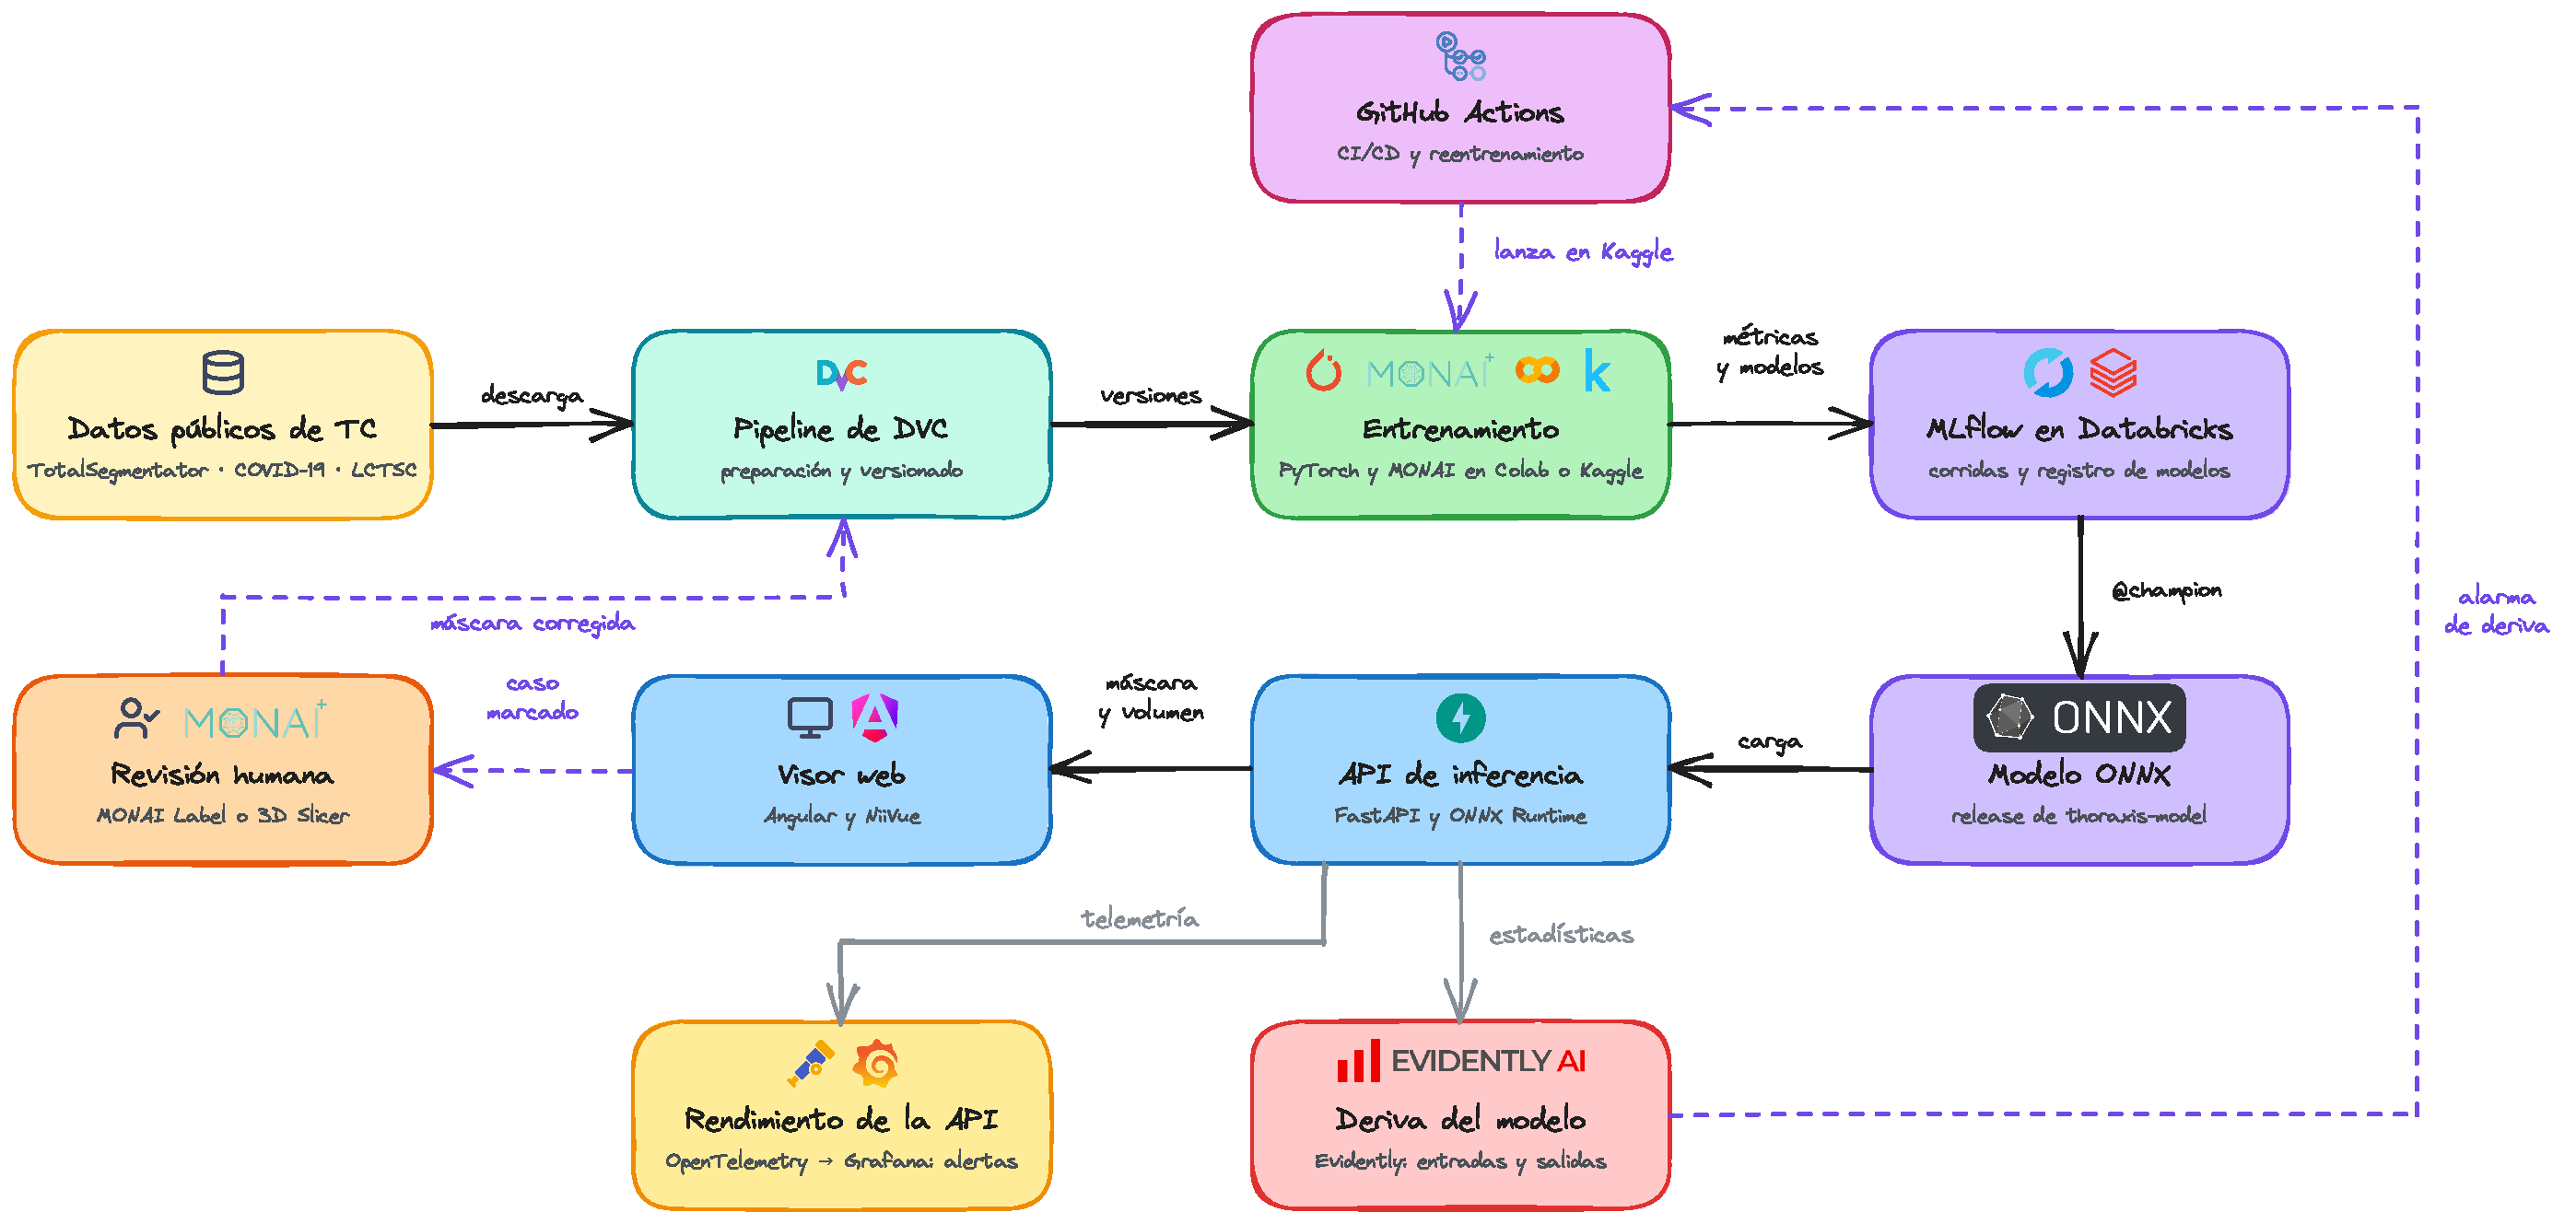
\includegraphics[width=\linewidth]{thoraxis-architecture}
    \articleSource{Elaboración propia con Excalidraw.}
\end{figure}
\end{landscape}}

El prototipo trabaja solo con estudios de los conjuntos públicos y muestra en
todo momento que se trata de una herramienta de investigación. Recibe estudios
en NIfTI, el formato de los datos procesados y de las máscaras. Los estudios
en DICOM, como los de LCTSC, se convierten antes a NIfTI; leerlos directamente
en el navegador, que NiiVue permite convirtiéndolos con dcm2niix compilado a
WebAssembly \parencite{niivuedicom}, queda como extensión futura.

% -----------------------------------------------------------------------------
% Explicabilidad. Afirmaciones verificadas en los resúmenes de cada fuente
% (Crossref, PubMed y Semantic Scholar) el 8 de noviembre de 2026.
% -----------------------------------------------------------------------------
\subsection{Explicabilidad e incertidumbre}\label{sec:explainability}
En imagen médica, la explicabilidad suele asociarse a los mapas de calor que
resaltan las regiones que más influyen en una predicción, como Grad-CAM. La
evidencia, sin embargo, desaconseja usarlos como explicación para el usuario.
En radiografías de tórax, siete de estos métodos, incluido Grad-CAM,
localizaron las patologías significativamente peor que un radiólogo, con la
mayor diferencia en lesiones pequeñas y de forma compleja
\parencite{saporta2022}. En otro estudio, los ocho métodos evaluados fallaron
al menos un criterio de confiabilidad, y varios no cambiaban al aleatorizar los
pesos del modelo, es decir, no reflejaban lo aprendido \parencite{arun2021}. Una
revisión de la explicabilidad en segmentación advierte además que las métricas
actuales para evaluar estos mapas son poco confiables \parencite{gipiskis2024}.

En segmentación resulta más útil mostrar cuánta confianza tiene el modelo en
cada vóxel. La cuantificación de la incertidumbre reduce el efecto de caja
negra de los modelos y hace sus resultados más interpretables y aceptables para
el usuario \parencite{lambert2024}. Las U-Net, en particular, tienden a dar
predicciones demasiado confiadas, tanto cuando aciertan como cuando se
equivocan \parencite{mehrtash2020}. Por eso Thoraxis explica sus segmentaciones
con tres componentes, que se describen con el marco de criterios de
\textcite{vandervelden2022}: todos son explicaciones locales, posteriores al
entrenamiento.

\begin{enumerate}
    \item \textbf{Mapa de incertidumbre por vóxel:} el modelo segmenta varias
          versiones del estudio con aumentos de datos aplicados durante la
          inferencia (\textit{test-time augmentation}), y la variación entre
          esas predicciones se muestra en el visor sobre los cortes. Esta
          técnica estima la incertidumbre mejor que el \textit{dropout} en la
          inferencia y reduce las predicciones erróneas con exceso de
          confianza \parencite{wang2019}; MONAI la implementa
          \parencite{cardoso2022}, por lo que no exige entrenar de nuevo.
    \item \textbf{Puntuación de confianza por caso:} un valor por estudio,
          derivado de la variación del volumen pulmonar entre esas
          predicciones. Los estudios con baja confianza se marcan para la
          revisión humana y la puntuación se envía al monitoreo
          (Sección~\ref{sec:continuous}). Un conjunto de varios modelos
          mejora la calibración de la confianza y permite predecir la calidad
          de la segmentación y detectar estudios distintos a los de
          entrenamiento \parencite{mehrtash2020}; queda como mejora opcional,
          porque multiplica el costo de entrenamiento.
    \item \textbf{Mapas de calor para uso interno:} Seg-Grad-CAM, la extensión
          de Grad-CAM a la segmentación \parencite{vinogradova2020}, se usa
          solo en el análisis de errores del equipo, acompañado de la prueba
          de aleatorizar los pesos del modelo, y no se presenta como
          explicación al usuario.
\end{enumerate}

La incertidumbre explica algo solo si anticipa los errores. Por eso su
evaluación forma parte de la evaluación de la solución
(Sección~\ref{sec:uncertainty-eval}). La inferencia con aumentos multiplica el
tiempo de respuesta por el número de versiones, de modo que el servicio la
ofrece como una opción de la consulta y no en cada predicción.

\subsection{Dudas de viabilidad}\label{sec:feasibility}
Estas son las principales dudas sobre la viabilidad de la propuesta, para
revisar en la primera asesoría:

\begin{enumerate}
    \item \textbf{Cómputo:} las sesiones de Colab duran como máximo 12~horas
          (24 en Pro+) y la GPU depende de la disponibilidad
          \parencite{colabpricing}. ¿Basta para entrenar la propuesta y las
          variantes del estudio de ablación, guardando puntos de control para
          reanudar el entrenamiento?
    \item \textbf{Almacenamiento:} TotalSegmentator ocupa 37,4~GB comprimido.
          ¿Conviene procesar una sola vez un subconjunto de estudios de tórax
          y guardar solo los volúmenes remuestreados?
    \item \textbf{Convenciones de etiquetado:} LCTSC excluye hilios, bronquios
          principales y, en la mayoría de los casos, el tumor
          (Sección~\ref{sec:data-limitations}). ¿Es aceptable fijar el
          criterio de éxito de Dice $\geq 0{,}95$ sobre esas máscaras, o
          conviene reportar también un análisis que separe el efecto de la
          convención?
    \item \textbf{2.5D frente a 3D:} ¿es suficiente el contexto de unos pocos
          cortes vecinos, o se espera comparar con un modelo 3D?
    \item \textbf{Estudios pediátricos:} ¿se incluyen los 291 estudios
          pediátricos de TotalSegmentator, aunque la validación externa sea
          solo con adultos?
    \item \textbf{Licencia del conjunto de COVID-19:} ¿basta con ajustarse a la
          licencia más restrictiva para su uso académico?
    \item \textbf{Entrenamiento continuo:} sin datos reales de pacientes, ¿es
          aceptable demostrarlo con lotes de datos y deriva simulados
          (Sección~\ref{sec:continuous}), y alcanza la cuota semanal gratuita
          de GPU de Kaggle para los reentrenamientos?
    \item \textbf{Compatibilidad de MONAI:} su versión vigente, la 1.6.1,
          declara compatibilidad oficial hasta Python~3.13, y el proyecto usa
          Python~3.14. ¿Conviene fijar Python~3.13 en el repositorio del modelo
          si MONAI no funciona con la versión más reciente?
\end{enumerate}

\subsection{Registro de experimentos y entorno}\label{sec:experiments}
Los experimentos se registran con MLflow \parencite{mlflow}, la plataforma de
código abierto que \textcite{kreuzberger2023} señalan como ejemplo de registro
de modelos y de almacén de metadatos. Cada corrida de entrenamiento guarda sus
parámetros, métricas, artefactos y la versión del código que la produjo, y los
modelos candidatos se versionan en el registro de modelos de MLflow, incluido
el modelo exportado a ONNX. El modelo elegido se publica además como versión
inmutable del repositorio \texttt{thoraxis-model}, que es la que consume el
servicio de inferencia.

El servidor de MLflow es el que ofrece Databricks Free Edition
\parencite{databricksfree}, un espacio de trabajo gratuito para uso no
comercial en el que los tres integrantes comparten los experimentos y el
registro de modelos de Unity Catalog. El entrenamiento corre fuera de
Databricks, en las máquinas del equipo o en Colab, y registra sus resultados
de forma remota con un token de acceso personal; los proyectos en Python se
gestionan con uv y Python~3.14, y MLflow guarda junto a cada modelo el
\texttt{uv.lock} con sus dependencias exactas. Antes de adoptarlo se verificó
desde una máquina local que el registro remoto de corridas y de modelos
funciona en esta edición, porque su documentación no lo especifica.

\pendiente{experimentos y cambios realizados con sus configuraciones
relevantes, versiones de librerías, semillas y recursos de cómputo utilizados}

% -----------------------------------------------------------------------------
% Ciclo de vida, cronograma y MLOps. Las fechas de los hitos salen de la guía
% (sección 4); los principios, de Kreuzberger et al. (2023), lectura del curso.
% Lo que aún no está decidido va como \pendiente.
% -----------------------------------------------------------------------------
\subsection{Ciclo de vida y MLOps}\label{sec:lifecycle}

\subsubsection{Ciclo de vida y cronograma}\label{sec:schedule}
El proyecto sigue un ciclo de vida iterativo, alineado con los tres avances y
la entrega final que fija la guía del proyecto integrador. Cada hito cierra una
iteración con un entregable revisable y una versión del repositorio
(Tabla~\ref{tab:schedule}).

\begin{table}[htbp]
    \centering
    \caption{Fases del ciclo de vida e hitos del proyecto.}\label{tab:schedule}
    \small
    \begin{tabularx}{\textwidth}{>{\raggedright\arraybackslash}p{3.3cm}
                                 >{\raggedright\arraybackslash}p{2.6cm}
                                 >{\raggedright\arraybackslash}X}
        \toprule
        Fase & Hito y fecha & Entregables \\
        \midrule
        Planificación y análisis & Asesoría 1: 6--13 nov 2026 &
            Problema, contexto y evidencia; objetivos; fuente de datos y forma
            de acceso; propuesta inicial y dudas de viabilidad. \\
        Diseño y desarrollo inicial & Asesoría 2: 7--11 dic 2026 &
            Datos preparados o muestra representativa; solución base y
            primeros resultados; diseño, métricas y procedimiento de
            evaluación. \\
        Desarrollo, pruebas e integración & Asesoría 3: 1--5 mar 2027 &
            Prototipo funcional; comparación con la solución base; análisis
            de errores y limitaciones; borrador del informe. \\
        Entrega y sustentación & 20 mar 2027 &
            Informe final, código e instrucciones, datos de prueba o acceso,
            diapositivas y demostración. \\
        \bottomrule
    \end{tabularx}
    \articleSource{Elaboración propia a partir de la guía del proyecto
    integrador.}
\end{table}

\pendiente{tareas por semana dentro de cada fase y responsable de cada una:
preparación de datos, desarrollo, evaluación y documentación}

\subsubsection{Prácticas de MLOps}\label{sec:mlops}
MLOps aplica al aprendizaje automático las prácticas de DevOps para llevar los
modelos a producción de forma automatizada y reproducible.
\textcite{kreuzberger2023} lo sintetizan en nueve principios, que sirven de
guía para el proyecto (Tabla~\ref{tab:mlops}).

\begin{table}[htbp]
    \centering
    \caption{Principios de MLOps y su aplicación en Thoraxis.}\label{tab:mlops}
    \small
    \begin{tabularx}{\textwidth}{>{\raggedright\arraybackslash}p{4.4cm}
                                 >{\raggedright\arraybackslash}X}
        \toprule
        Principio & Práctica en Thoraxis \\
        \midrule
        Automatización de CI/CD & GitHub Actions en cada repositorio: lint,
            pruebas y compilación en cada cambio; versiones con
            release-please. \\
        Orquestación de flujos & Pipeline de DVC con las etapas de
            preparación, entrenamiento, evaluación y exportación, lanzado por
            GitHub Actions en Kaggle. \\
        Reproducibilidad & Plantilla ReproPath en el repositorio del modelo;
            semillas y versiones de librerías fijadas. \\
        Versionado de datos, código y modelo & Código en Git; modelos
            candidatos en el registro de modelos de MLflow; modelo ONNX elegido
            publicado como versión inmutable del repositorio; datos procesados
            versionados con DVC. \\
        Colaboración & Repositorios separados por componente, cambios por pull
            request y revisión entre integrantes. \\
        Entrenamiento y evaluación continuos & Reentrenamiento en Kaggle ante
            datos nuevos o una alarma del monitoreo; cada modelo se evalúa y
            solo se promueve si mejora al vigente
            (Sección~\ref{sec:continuous}). \\
        Seguimiento de metadatos & MLflow Tracking: parámetros, métricas,
            artefactos y versión del código de cada corrida de
            entrenamiento. \\
        Monitoreo continuo & Del modelo: Evidently en el servicio de
            inferencia, para detectar cambios en las estadísticas de entrada y
            de salida. Del aplicativo: OpenTelemetry y Grafana, para la
            latencia, los errores y el uso de recursos de la API. \\
        Ciclos de retroalimentación & Del monitoreo al reentrenamiento, del
            análisis de errores a la preparación de datos y de la revisión
            humana a los datos. \\
        \bottomrule
    \end{tabularx}
    \articleSource{Elaboración propia a partir de
    \textcite{kreuzberger2023}.}
\end{table}

% -----------------------------------------------------------------------------
% Contraste de herramientas. Precios y límites consultados el 8 de noviembre
% de 2026 en las páginas oficiales; revisarlos antes de cada entrega, porque
% cambian sin aviso.
% -----------------------------------------------------------------------------
\subsubsection{Herramientas de MLOps}\label{sec:mlops-tools}
El servidor de MLflow se eligió entre tres opciones: un servidor local,
DagsHub y Databricks. Un servidor local no permite que los tres integrantes
compartan los experimentos, así que la comparación se centró en los dos
servicios gestionados (Tabla~\ref{tab:mlflow-hosting}). Ambos ejecutan MLflow
estándar: el código de entrenamiento es el mismo y solo cambian la dirección
del servidor y las credenciales, de modo que cambiar de servicio más adelante
no obliga a reescribirlo.

\begin{table}[htbp]
    \centering
    \caption{Opciones de alojamiento del servidor de MLflow.}%
    \label{tab:mlflow-hosting}
    \small
    \begin{tabularx}{\textwidth}{>{\raggedright\arraybackslash}p{2.8cm}
                                 >{\raggedright\arraybackslash}X
                                 >{\raggedright\arraybackslash}X
                                 >{\raggedright\arraybackslash}X}
        \toprule
        Criterio & DagsHub (plan gratuito) & Databricks Free Edition &
            Databricks de pago \\
        \midrule
        Costo & Gratis. & Gratis. & Pago por uso en DBU, sin licencia fija;
            prueba de 14 días con hasta 400~USD de crédito. \\
        Equipo de tres & Repositorio público: colaboradores ilimitados.
            Privado: el dueño y dos colaboradores. & Un espacio de trabajo por
            cuenta, compartido con los integrantes invitados. & Sin límite
            relevante. \\
        Experimentos & Repositorio público: ilimitados y visibles para
            cualquiera. Privado: hasta 100. & Sin límite publicado; cuota
            diaria de uso sin cifra publicada. & Según el consumo. \\
        Almacenamiento & 20~GB (la misma página indica también 200~GB). &
            No publicado. & Según el proveedor de nube. \\
        GPU para entrenar & No ofrece cómputo. & Acceso limitado a AI Runtime
            si se verifica la cuenta con LinkedIn. & Clústeres con GPU o AI
            Runtime, con costo por hora (Tabla~\ref{tab:gpu-costs}). \\
        Registro desde PC o Colab & Documentado. & Verificado por el equipo.
            & Documentado. \\
        Uso & No comercial en repositorios privados. & Solo no comercial. &
            Sin restricción. \\
        Riesgos & Experimentos públicos si el repositorio es público. &
            Elimina cuentas inactivas por un período prolongado; sin soporte.
            & Costo variable según el uso. \\
        \bottomrule
    \end{tabularx}
    \articleSource{Elaboración propia a partir de \textcite{dagshubpricing},
    \textcite{databricksfree} y \textcite{databrickspricing}.}
\end{table}

Se eligió Databricks Free Edition porque no limita el número de experimentos,
los mantiene privados al equipo e incluye el registro de modelos de Unity
Catalog; además, Databricks figura entre las plataformas comerciales de MLOps
que revisan \textcite{kreuzberger2023}. Sus riesgos, la cuota diaria y la
posible eliminación de cuentas inactivas, se acotan porque el modelo elegido
se publica en \texttt{thoraxis-model} y el código no depende del servicio.

Para registrar experimentos, el plan de pago de Databricks no aporta nada sobre
el gratuito. La plataforma no cobra una licencia mensual, sino el cómputo
consumido: en AWS, plan Premium y región US East, el cómputo interactivo
\textit{serverless} cuesta 0{,}75~USD por DBU y los trabajos
\textit{serverless}, 0{,}35~USD por DBU, con la infraestructura incluida
\parencite{databrickspricing, databricksjobs}. MLflow gestionado viene incluido
en ese cómputo y no tiene una tarifa propia publicada. El plan Team de DagsHub
cuesta 99~USD por usuario al mes con pago anual y 119~USD con pago mensual
\parencite{dagshubpricing}, es decir, entre 297 y 357~USD al mes para tres
integrantes. Por eso el registro de experimentos se mantiene en el plan
gratuito.

El entrenamiento con GPU es otro asunto. El equipo entrena en Google Colab,
que cobra por unidades de cómputo: el plan Pro cuesta 9{,}99~USD al mes con
100 unidades y el Pro+, 49{,}99~USD con 600; las unidades vencen a los 90
días, y Pro+ mantiene la ejecución hasta 24~horas con el navegador cerrado
\parencite{colabpricing}. Google no publica cuántas unidades por hora consume
cada GPU, y las GPU disponibles dependen de la demanda. Databricks ofrece dos
alternativas de pago (Tabla~\ref{tab:gpu-costs}). En los clústeres clásicos, la
máquina con GPU se paga a AWS y los DBU a Databricks, lo que exige una cuenta
propia de AWS \parencite{databrickscalculator, awsec2}. AI Runtime, en vista
previa, cobra un precio único por hora de GPU con la infraestructura incluida
\parencite{databricksairuntime}. Free Edition, por su parte, da acceso limitado
a AI Runtime si se verifica la cuenta con LinkedIn, sin publicar cuántas horas
\parencite{databricksfree}.

\begin{table}[htbp]
    \centering
    \caption{Costo del entrenamiento con GPU en Databricks.}%
    \label{tab:gpu-costs}
    \small
    \begin{tabularx}{\textwidth}{>{\raggedright\arraybackslash}X
                                 >{\raggedright\arraybackslash}p{2.6cm}
                                 >{\raggedright\arraybackslash}p{2.2cm}
                                 >{\raggedright\arraybackslash}p{2.2cm}}
        \toprule
        Opción & GPU & USD por hora & 100~horas al mes \\
        \midrule
        Clásico, como trabajo & T4 (16~GB) & 0{,}63 & 63~USD \\
        Clásico, como trabajo & A10G (24~GB) & 1{,}21 & 121~USD \\
        Clásico, en notebook interactivo & A10G (24~GB) & 1{,}75 & 175~USD \\
        AI Runtime (vista previa) & A10 (24~GB) & 2{,}50 & 250~USD \\
        AI Runtime (vista previa) & H100 (80~GB) & 7{,}00 & 700~USD \\
        AI Runtime en Free Edition & Sin publicar & Gratis, con acceso
            limitado & Sin publicar \\
        \bottomrule
    \end{tabularx}
    \articleSource{Elaboración propia a partir de
    \textcite{databrickscalculator}, \textcite{awsec2},
    \textcite{databricksairuntime} y \textcite{databricksfree}. AWS, plan
    Premium, región US East; el costo clásico suma la instancia de AWS
    (\texttt{g4dn.xlarge} y \texttt{g5.xlarge}) y los DBU de Databricks.}
\end{table}

Para el desarrollo se mantiene Colab para entrenar y Databricks Free Edition
para registrar los experimentos. Pagar Databricks se justificaría solo si
Colab no alcanza, por ejemplo con entrenamientos de más de 24~horas o si se
necesita una GPU garantizada; en ese caso, AI Runtime evita administrar una
cuenta de AWS, y la prueba gratuita de 14 días incluye hasta 400~USD de crédito
\parencite{databrickstrial}.
\pendiente{horas de GPU estimadas por mes y acceso a AI Runtime obtenido con la
verificación de Free Edition}

MLflow sobre Databricks cubre solo una parte de los principios de la
Tabla~\ref{tab:mlops}. La Tabla~\ref{tab:mlflow-coverage} contrasta qué
resuelve y qué queda a cargo de otras herramientas.

\begin{table}[htbp]
    \centering
    \caption{Cobertura de MLflow sobre Databricks frente a los principios de
    MLOps.}\label{tab:mlflow-coverage}
    \small
    \begin{tabularx}{\textwidth}{>{\raggedright\arraybackslash}p{4.4cm}
                                 >{\raggedright\arraybackslash}p{1.7cm}
                                 >{\raggedright\arraybackslash}X}
        \toprule
        Principio & Cobertura & Detalle \\
        \midrule
        Seguimiento de metadatos & Completa & MLflow Tracking registra
            parámetros, métricas, artefactos y el commit de cada corrida. \\
        Versionado del modelo & Completa & El registro de Unity Catalog
            versiona cada modelo; un alias como \texttt{@champion} marca el
            elegido. \\
        Versionado de datos & Parcial & \texttt{mlflow.log\_input} guarda una
            huella del conjunto usado en cada corrida, sin copiar los datos. \\
        Reproducibilidad & Parcial & Cada modelo registrado guarda el
            \texttt{uv.lock}, los parámetros y el commit; las semillas y
            ReproPath dependen del código. \\
        Colaboración & Parcial & Espacio de trabajo compartido por los tres
            integrantes; la revisión de código sigue en GitHub. \\
        Automatización de CI/CD & Ninguna & GitHub Actions; un flujo puede
            consultar el registro para saber qué versión publicar. \\
        Orquestación de flujos & Ninguna & DVC y GitHub Actions; Databricks
            ofrece trabajos programados, pero el entrenamiento corre en Colab y
            Kaggle. \\
        Monitoreo continuo & Ninguna & Evidently, OpenTelemetry y Grafana en
            \texttt{thoraxis-api}; el monitoreo de Databricks está pensado para
            modelos servidos en la propia plataforma. \\
        Entrenamiento continuo y retroalimentación & Parcial & Los alias del
            registro distinguen el modelo candidato del vigente; el
            reentrenamiento corre en Kaggle y lo disparan GitHub Actions y
            Evidently. \\
        \bottomrule
    \end{tabularx}
    \articleSource{Elaboración propia a partir de \textcite{mlflow} y
    \textcite{kreuzberger2023}.}
\end{table}

% -----------------------------------------------------------------------------
% Entrenamiento continuo y retroalimentación (principios de Kreuzberger et al.,
% 2023). Herramientas y cuotas verificadas el 8 de noviembre de 2026.
% -----------------------------------------------------------------------------
\subsubsection{Entrenamiento continuo y retroalimentación}\label{sec:continuous}
Según \textcite{kreuzberger2023}, el entrenamiento continuo reentrena el modelo
cuando hay datos nuevos, se apoya en el monitoreo, en un ciclo de
retroalimentación y en un pipeline automatizado, y siempre incluye una
evaluación del cambio en la calidad del modelo. Los ciclos de
retroalimentación, por su parte, llevan lo aprendido en la evaluación de
vuelta al desarrollo, y lo observado en el monitoreo, al disparador del
reentrenamiento.

\paragraph{Dónde se reentrena.}
Colab no ofrece una forma gratuita de programar ejecuciones: la programación es
una función de Colab Enterprise, un servicio de pago de Google Cloud
\parencite{colabschedule}. GitHub Actions ofrece máquinas con GPU T4 a
0,052~USD por minuto, pero solo para organizaciones con planes de pago
\parencite{githubrunners}. Por eso el reentrenamiento automático corre en
Kaggle Notebooks, que ofrece gratis una GPU P100 o dos T4, con sesiones de
hasta 12~horas y una cuota semanal, y permite programar ejecuciones o
dispararlas cuando se actualiza un conjunto de datos \parencite{kagglenotebooks}.
Su interfaz de línea de comandos, además, lanza un notebook con GPU desde un
flujo de GitHub Actions \parencite{kagglecli}. Colab se mantiene para la
experimentación interactiva.

\paragraph{Flujo de reentrenamiento.}
\begin{enumerate}
    \item \textbf{Disparo:} una versión nueva de los datos procesados, que se
          versionan con DVC \parencite{dvc}, o una alarma del monitoreo.
    \item \textbf{Ejecución:} GitHub Actions lanza en Kaggle el pipeline de
          DVC, con las etapas de preparación, entrenamiento, evaluación y
          exportación, y la corrida queda registrada en MLflow.
    \item \textbf{Evaluación:} el modelo nuevo se evalúa en la prueba interna
          fija y en LCTSC, y se registra en Unity Catalog con el alias
          \texttt{@challenger} \parencite{databricksaliases}.
    \item \textbf{Promoción:} un control en GitHub Actions lo compara con el
          modelo vigente, identificado con el alias \texttt{@champion}. Solo
          si lo supera y cumple el criterio de éxito
          (Sección~\ref{sec:expected-outcome}) recibe ese alias, y su versión
          ONNX se publica en \texttt{thoraxis-model} tras la aprobación de un
          integrante.
\end{enumerate}

\paragraph{Ciclos de retroalimentación.}
Thoraxis implementa tres:

\begin{itemize}
    \item \textbf{Del monitoreo al reentrenamiento:} el servicio de inferencia
          registra con Evidently solo estadísticas de cada estudio, nunca las
          imágenes: a la entrada, el espaciado, el espesor de corte y los
          percentiles de intensidad; a la salida, el volumen de cada pulmón,
          la relación entre ambos, el número de fragmentos y la puntuación de
          confianza. Evidently
          convierte la comparación con los datos de referencia en pruebas que
          pasan o fallan \parencite{evidently}; si fallan, GitHub Actions
          dispara el reentrenamiento.
    \item \textbf{De la evaluación al desarrollo:} los casos de error del
          análisis (Sección~\ref{sec:errors}) vuelven a la preparación de
          datos, por ejemplo para incorporar más pulmones con patología.
    \item \textbf{De la revisión humana a los datos:} en el visor, un revisor
          marca una segmentación incorrecta, o el sistema marca una de baja
          confianza (Sección~\ref{sec:explainability}); el caso se corrige en
          MONAI
          Label, un marco de anotación interactiva asistida por IA para
          imágenes médicas 3D \parencite{diazpinto2024}, y la máscara
          corregida entra en una versión nueva de los datos, que dispara el
          reentrenamiento. La última versión publicada de MONAI Label es de
          octubre de 2023, aunque su repositorio sigue recibiendo cambios; si
          no funciona con el entorno del proyecto, las correcciones se harán a
          mano en 3D Slicer.
\end{itemize}

El proyecto no recibe datos de pacientes, así que no llegarán datos nuevos por
sí solos. Para demostrar los ciclos se simulan: una parte de los estudios de
TotalSegmentator se reserva como datos futuros que llegan por lotes, y la
deriva se simula con estudios de otra fuente o con cortes más gruesos. Los
resultados se presentarán como una demostración del mecanismo, no como un
sistema en operación. La Figura~\ref{fig:architecture} resume el flujo
completo, de los datos al visor web, junto con los tres ciclos de
retroalimentación.

% -----------------------------------------------------------------------------
% Monitoreo del aplicativo. Límites del plan gratuito de Grafana Cloud y versión
% de la instrumentación de FastAPI verificados el 8 de noviembre de 2026.
% -----------------------------------------------------------------------------
\subsubsection{Monitoreo del aplicativo}\label{sec:app-monitoring}
Evidently vigila el modelo, pero no si el servicio responde a tiempo. Para eso
la API se instrumenta con OpenTelemetry, un marco de código abierto para
generar, recolectar y exportar trazas, métricas y registros sin depender de un
proveedor. OpenTelemetry no guarda ni muestra los datos: deja esas tareas a
otras herramientas \parencite{opentelemetry}. Su instrumentación para FastAPI
mide cada petición de forma automática, y su versión 0.66b2, todavía en
fase beta, declara compatibilidad con Python~3.14 \parencite{otelfastapi}. La
API emite tres tipos de datos:

\begin{itemize}
    \item \textbf{Métricas:} peticiones por minuto, tasa de errores y latencia
          de cada endpoint, más métricas propias del proyecto: el tiempo de
          preprocesamiento, el de inferencia con ONNX Runtime, el de la
          inferencia con aumentos para el mapa de incertidumbre y la memoria
          del proceso.
    \item \textbf{Trazas:} cada consulta se divide en tramos (carga del
          estudio, preprocesamiento, inferencia y posprocesamiento), lo que
          permite ubicar la etapa lenta.
    \item \textbf{Registros:} los errores, con el identificador de su traza.
          Igual que en Evidently, solo se registran metadatos, nunca las
          imágenes.
\end{itemize}

Los datos se envían a Grafana Cloud, que recibe OpenTelemetry directamente. Su
plan gratuito incluye 10\,000 series activas de métricas, 50~GB de registros y
50~GB de trazas al mes, con 14~días de retención, y hasta tres usuarios
activos, el tamaño del equipo \parencite{grafanapricing}. En Grafana se arma un
panel con el rendimiento de la API y alertas que avisan al equipo cuando la
latencia o la tasa de errores superan un umbral. A diferencia de las pruebas de
Evidently, estas alertas no disparan el reentrenamiento, porque un problema de
rendimiento no se resuelve reentrenando el modelo. Las mismas mediciones
alimentan la evaluación del tiempo de respuesta y de los recursos
(Sección~\ref{sec:resources}); como la retención es de 14~días, se exportan al
terminar cada evaluación. El visor web no se instrumenta, porque el costo
está en la API.

\subsection{Material técnico y reproducibilidad}\label{sec:repositories}
El código del proyecto se organiza en cuatro repositorios:

\begin{itemize}
    \item \textbf{Modelo:} entrenamiento, evaluación y exportación.
          \url{https://github.com/ahincho/thoraxis-model}
    \item \textbf{API:} servicio de inferencia.
          \url{https://github.com/ahincho/thoraxis-api}
    \item \textbf{Web:} visor de cortes con la máscara de segmentación.
          \url{https://github.com/ahincho/thoraxis-web}
    \item \textbf{Informe:} este documento.
          \url{https://github.com/ahincho/thoraxis-article}
\end{itemize}

\pendiente{instrucciones para reproducir la evaluación y acceso a los datos de
prueba}

% !TEX root = ../article.tex
% =============================================================================
% 3.6 Evaluación de la solución
% =============================================================================
% Guía: métricas y criterios adecuados para la tarea, con su justificación;
% comparación entre la solución base y la propuesta en las mismas
% condiciones; resultados con tablas, gráficos y ejemplos de aciertos y
% errores; tiempo de respuesta, consumo de recursos o costo cuando sean
% relevantes. Debe incluir casos representativos del uso previsto.
%
% Segundo avance (asesoría 2, 7-11 dic 2026): diseño de la solución,
% métricas y procedimiento de evaluación; solución base y primeros
% resultados.
% =============================================================================

\section{Evaluación de la solución}\label{sec:evaluation}

\subsection{Métricas y criterios}\label{sec:metrics}
\pendiente{métricas de segmentación elegidas y por qué son adecuadas}

\subsection{Comparación con la solución base}\label{sec:comparison}
\pendiente{tabla con la solución base y la propuesta, evaluadas sobre el mismo
conjunto de prueba}

% Plantilla de tabla (descomentar cuando haya resultados):
% \begin{table}[htbp]
%     \centering
%     \caption{Comparación entre la solución base y la propuesta.}\label{tab:comparison}
%     \begin{tabular}{lcc}
%         \toprule
%         Modelo & Métrica 1 & Métrica 2 \\
%         \midrule
%         Solución base & -- & -- \\
%         Propuesta     & -- & -- \\
%         \bottomrule
%     \end{tabular}
%     \articleSource{Elaboración propia.}
% \end{table}

\subsection{Ejemplos de aciertos y errores}\label{sec:examples}
\pendiente{casos representativos del uso previsto: cortes con la máscara
predicha frente a la de referencia, incluidos casos de fallo}

\subsection{Evaluación de la incertidumbre}\label{sec:uncertainty-eval}
La incertidumbre (Sección~\ref{sec:explainability}) se evalúa con el mismo
conjunto de prueba interno y con la validación externa, en tres pruebas:

\begin{enumerate}
    \item \textbf{Relación con el error por caso:} correlación de Spearman
          entre la puntuación de confianza de cada estudio y su Dice. Una
          correlación clara indica que la puntuación sirve para marcar los
          casos que requieren revisión.
    \item \textbf{Relación con el error por vóxel:} capacidad del mapa de
          incertidumbre para distinguir los vóxeles mal segmentados de los
          bien segmentados, medida con el área bajo la curva ROC.
    \item \textbf{Calibración:} diagrama de confiabilidad que compara las
          probabilidades del modelo con la proporción real de aciertos, porque
          las U-Net tienden a ser demasiado confiadas \parencite{mehrtash2020}.
\end{enumerate}

\pendiente{resultados de las tres pruebas, con la solución base y la
propuesta}

\subsection{Tiempo de respuesta y recursos}\label{sec:resources}
\pendiente{tiempo de inferencia por estudio, memoria y costo de uso}

% !TEX root = ../article.tex
% =============================================================================
% 3.7 Resultados y discusión
% =============================================================================
% Guía: interpretación de los resultados en relación con los objetivos;
% errores frecuentes, casos en que la solución falla y posibles causas;
% limitaciones técnicas, riesgos y consideraciones éticas; condiciones
% necesarias para aplicar la solución y mejoras pendientes.
%
% Tercer avance (asesoría 3, 1-5 mar 2027): análisis de errores,
% limitaciones y aspectos pendientes.
% =============================================================================

\section{Resultados y discusión}\label{sec:discussion}

\subsection{Interpretación frente a los objetivos}\label{sec:interpretation}
\pendiente{qué dicen los resultados respecto de cada objetivo}

\subsection{Análisis de errores}\label{sec:errors}
\pendiente{errores frecuentes, casos en los que el modelo falla y posibles
causas}

\subsection{Limitaciones, riesgos y consideraciones éticas}\label{sec:ethics}
\pendiente{limitaciones técnicas, riesgos y consideraciones éticas; uso solo
para investigación y no para diagnóstico}

\subsection{Condiciones de uso y trabajo futuro}\label{sec:future-work}
\pendiente{condiciones necesarias para aplicar la solución y mejoras
pendientes}

% !TEX root = ../article.tex
% =============================================================================
% 3.8 Conclusiones
% =============================================================================
% Guía: hallazgos principales, en qué medida se cumplieron los objetivos y
% utilidad de la solución en el contexto elegido. Deben apoyarse en los
% resultados obtenidos.
% =============================================================================

\section{Conclusiones}\label{sec:conclusions}

\pendiente{hallazgos principales, grado de cumplimiento de cada objetivo y
utilidad de Thoraxis en el contexto elegido, apoyados en los resultados}


% --- Referencias (IEEE) ---
% La guía pide incluir fuentes bibliográficas, conjuntos de datos, modelos,
% documentación y código de terceros, con un mismo formato de citación.
\section*{Referencias}
\addcontentsline{toc}{section}{Referencias}
\printbibliography[heading=none]

\end{document}
